\chapter{Apartado A: \textbf{Segmentación por color}}
\label{chapter:tarea_a}

En este apartado deberá segmentar los colores blancos y naranjas que aparecen en las imágenes disponibles en la carpeta \texttt{data}. Segmentar por colores es una técnica sencilla y útil en aplicaciones en las que se tiene un gran control sobre las condiciones de contorno: iluminación, tipo de objeto que se espera encontrar, color del fondo, etc. A continuación se añaden algunos comentarios para resolver paso a paso la tarea:

\section*{Tarea A.1: Carga de imágenes}
\phantomsection
\addcontentsline{toc}{section}{Tarea A.1: Carga de imágenes}

Para trabajar de forma eficiente, antes de empezar a procesar imágenes deberá definir algunos métodos auxiliares. El primero de ellos es un método que debe cargar imágenes de la carpeta \texttt{data}.

\section*{Tarea A.2: Visualización y guardado de imágenes}
\addcontentsline{toc}{section}{Tarea A.2: Visualización y guardado de imágenes}

De nuevo, estos métodos ya los utilizó en la 1ª sesión de laboratorio, así que aproveche este paso para afianzar conceptos. Defina los métodos para visualizar imágenes y guardarlas. Respete y utilice todos los argumentos que se proporcionan.

\section*{Tarea A.3: Cambio de espacio de color}
\addcontentsline{toc}{section}{Tarea A.3: Cambio de espacio de color}

Cambie el espacio de color de las imágenes (BGR) a uno donde la crominancia e intensidad estén separados (HSV). Puede interpretar este paso como un cambio de sistema de referencia (cartesiano a polar). De esta forma, le será más fácil discriminar los colores de interés. La Figura \ref{fig:color_spaces} \footnote{ \href{https://commons.wikimedia.org/wiki/File:RGB\_2\_HSV\_conversion\_with\_grid.ogg}{Imagen modificada de VerbaGleb, CC BY-SA 4.0} https://commons.wikimedia.org/wiki/File:RGB\_2\_HSV\_conversion\_with\_grid.ogg} muestra los espacios de colores con los que trabajará.

Para cambiar el espacio de color de sus imágenes, puede utilizar el método \texttt{cv2.cvtColor()} de OpenCV. Tenga en cuenta que OpenCV cuenta con una gran cantidad de espacios de color, visite la documentación. \footnote{ \href{https://docs.opencv.org/3.4/d8/d01/group\_\_imgproc\_\_color\_\_conversions.html}{Espacios de color de OpenCV} https://docs.opencv.org/3.4/d8/d01/group\_\_imgproc\_\_color\_\_conversions.html}



\begin{figure}[h]
    \centering
    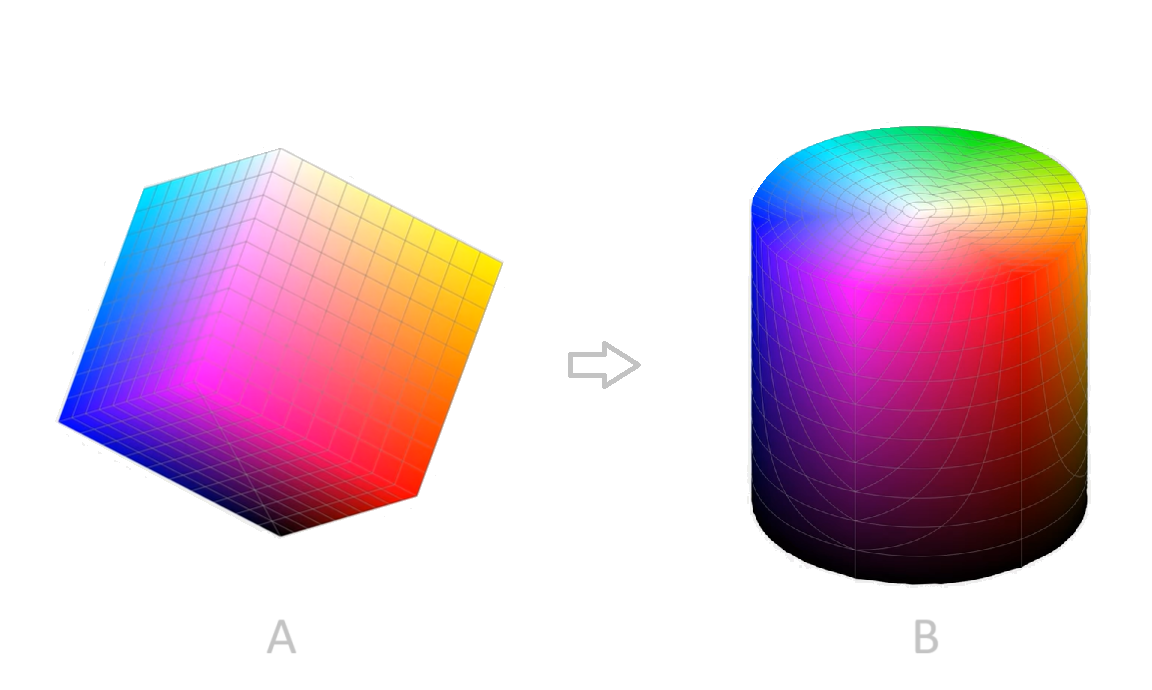
\includegraphics[width=0.5\textwidth]{Lab_2/template/figures/color_spaces.png}
    \caption{Espacios de color utilizados. Gráfico A: BGR (atención con el orden de canales en OpenCV) y Gráfico B: HSV.}
    
    \label{fig:color_spaces}
\end{figure}

\section*{Tarea A.4: Segmentación de las partes naranjas}
\addcontentsline{toc}{section}{Tarea A.4: Segmentación de las partes naranjas}

Genere una máscara para cada imagen y realice una segmentación con ella. Una máscara es una imagen binaria (blanca y/o negro) donde los píxeles de interés aparecen en blanco, mientras que los píxeles que no son de interés aparecen en negro. Segmentar implica multiplicar la imagen original con la máscara. Así se obtienen los píxeles de interés de la imagen original.

Para obtener las máscaras y segmentar la imagen, puede utilizar respectivamente los métodos \texttt{cv2.inRange()} y \texttt{cv2.bitwise\_and()} de OpenCV. Por otro lado, en este paso se facilitan los rangos de color naranja:

\begin{tcolorbox}[colback=gray!85, coltext=white, colframe=white, fonttitle=\bfseries, title=Important Note, boxrule=0.5mm]
\texttt{light\_orange = (1, 190, 200)}\\
\texttt{dark\_orange = (255, 255, 255)}
\end{tcolorbox}

Para confirmar que está obteniendo los resultados adecuados, muestre una de las imágenes iniciales, su máscara y la imagen segmentada.


\begin{figure}[h]
    \centering
    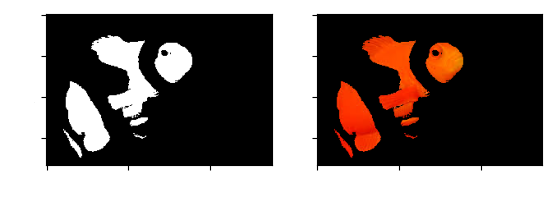
\includegraphics[width=0.5\textwidth]{Lab_2/template/figures/orange.png}
    \caption{Máscara y segmentación de colores naranjas.}
    \label{fig:orange_mask}
\end{figure}

\section*{Tarea A.5: Segmentación de las partes blancas}
\addcontentsline{toc}{section}{Tarea A.5: Segmentación de las partes blancas}

En este paso deberá repetir un proceso similar al anterior, pero centrándose en los tonos blancos. Explore el rango de valores necesarios para segmentar los colores blancos de las imágenes. Para ello, juegue con los valores de H, S y V en la interfaz que se le proporciona.

De nuevo, para confirmar que está obteniendo los resultados adecuados, muestre la máscara y la imagen segmentada.

\begin{figure}[h]
    \centering
    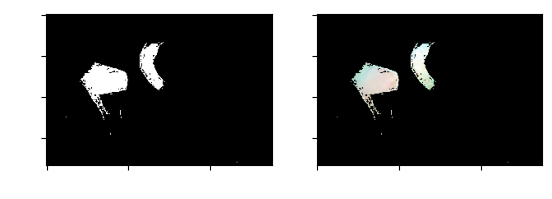
\includegraphics[width=0.5\textwidth]{Lab_2/template/figures/white.png}
    \caption{Máscara y segmentación de colores blancos.}
    \label{fig:whithe_mask}
\end{figure}

\section*{Tarea A.6: Combinación de máscaras}
\addcontentsline{toc}{section}{Tarea A.6: Combinación de máscaras}

Combine las máscaras de los colores naranja y blanco para cada imagen. Posteriormente, segmente cada imagen con la máscara que ha generado. Como resultado, conseguirá segmentar el cuerpo de los peces en el conjunto imágenes. Debería obtener resultados parecidos al ejemplo de la Figura \ref{fig:fish_output}.

Confirme que está obteniendo los resultados adecuados mostrando la máscara y la imagen segmentada.


\begin{figure}[h]
    \centering
    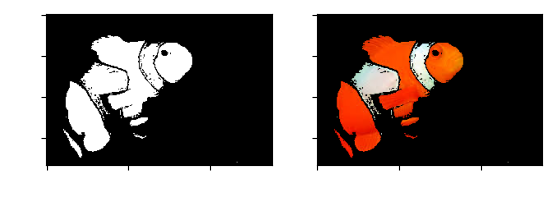
\includegraphics[width=0.5\textwidth]{Lab_2/template/figures/output.png}
    \caption{Máscara completa y segmentación del pez como combinación de colores blancos y naranjas.}
    \label{fig:fish_output}
\end{figure}


\section*{Tarea A.7: Guardado de imágenes}
\addcontentsline{toc}{section}{Tarea A.7: Guardado de imágenes}

Guarde las imágenes de interés como resultado de esta parte de la práctica.

\section*{Preguntas}
\addcontentsline{toc}{section}{Preguntas}

\vspace{5mm}
\begin{tcolorbox}[colback=gray!10, colframe=gray!30, coltitle=black, title=Pregunta A.1, halign=left]
Segmente por color el escudo de su equipo deportivo favorito: descompóngalo en al menos 2 colores. De igual forma que ha realizado en el ejercicio de clase, proporcione las máscaras binarias de cada color. Además, multiplique la máscara con la imagen original para visualizar solamente el color de interés. Por último indique el porcentaje que representa cada color sobre el total del escudo.
\end{tcolorbox}

\vspace{5mm}
\begin{tcolorbox}[colback=gray!10, colframe=gray!30, coltitle=black, title=Pregunta A.2, halign=left]
¿Qué ocurre cuando carga las imágenes con la librería \texttt{imageio} pero las visualiza con la librería \texttt{OpenCV}? Investigue qué puede estar pasando y cómo podría solucionarlo. Pista: cv2.cvtColor().
\end{tcolorbox}